\section{Dangers du milieu et environnement}

\begin{frame}{Dangers liés à la faune}
  \begin{itemize}
    \item Animaux qui \textbf{mordent} : murènes, congres…
    \item Animaux qui \textbf{piquent} : oursins, vives, certaines étoiles de mer, raies…
    \item Animaux qui \textbf{brûlent} : méduses, anémones de mer.
  \end{itemize}

  \begin{block}{Prévention}
    \begin{itemize}
      \item Ne pas \textbf{toucher} les animaux.
      \item Faire attention où l'on \textbf{pose les mains et les genoux}.
      \item Ne pas passer derrière une méduse (filaments parfois très longs).
    \end{itemize}
  \end{block}
\end{frame}

\begin{frame}{Autres dangers du milieu}
  \begin{itemize}
    \item \textbf{Courants} :
          \begin{itemize}
            \item Risque de s'éloigner du bateau.
            \item Nager à contre-courant $\Rightarrow$ essoufflement.
          \end{itemize}
    \item \textbf{Eaux troubles} :
          \begin{itemize}
            \item Risque de perte de la palanquée.
            \item Rester \textbf{regroupés côte à côte}.
          \end{itemize}
    \item \textbf{Grottes, tunnels, épaves} :
          \begin{itemize}
            \item Visibilité réduite, risque de rester coincé.
            \item Ne pas enlever son masque dans les grottes.
            \item Ne pas rentrer dans les épaves.
          \end{itemize}
    \item \textbf{Filets, cordages} :
          \begin{itemize}
            \item Risque d'emmêlement.
            \item Ne pas se débattre, appeler le coéquipier.
          \end{itemize}
  \end{itemize}
\end{frame}

\begin{frame}{Embarcations et parachute}
  \begin{itemize}
    \item Risque de \textbf{collision} avec des bateaux.
    \item Toujours regarder (360°) et écouter avant de faire surface.
    \item Le \textbf{parachute de palier}, géré par le guide, est un élément de sécurité.
  \end{itemize}
\end{frame}

\begin{frame}{Protection de l'environnement}
  \begin{itemize}
    \item L'écosystème sous-marin est \textbf{fragile}.
    \item Ne pas \textbf{palmer en raclant le fond} : les palmes sont l'ennemi n°1 de la faune et de la flore.
    \item Ne pas arracher coraux, gorgones, etc.
    \item Regarder, mais \textbf{ne pas toucher}.
    \item Ne pas perturber les animaux, surtout en période de reproduction.
    \item Ne tuer aucun animal : nous sommes des \textbf{invités} dans ce milieu.
  \end{itemize}
\end{frame}

\begin{frame}{Sons, couleurs et dimensions sous l'eau}
  \begin{columns}
    \column{0.5\textwidth}
    \begin{itemize}
      \item \textbf{Sons} :
        \begin{itemize}
          \item Ils se propagent plus vite dans l'eau.
          \item \textbf{Difficile de localiser} la provenance (avant / arrière, gauche / droite).
        \end{itemize}
      \item \textbf{Couleurs} :
        \begin{itemize}
          \item Le rouge disparaît dès \textbf{5–10 m}, puis l'orange, le jaune, etc.
          \item Tout paraît plus \textbf{bleu / vert} avec la profondeur.
        \end{itemize}
      \item \textbf{Dimensions} :
        \begin{itemize}
          \item Les objets paraissent \textbf{plus gros et plus proches} (effet masque + eau).
          \item Attention à l'\textbf{estimation des distances} et des tailles.
        \end{itemize}
    \end{itemize}

    \column{0.5\textwidth}
    \centering
    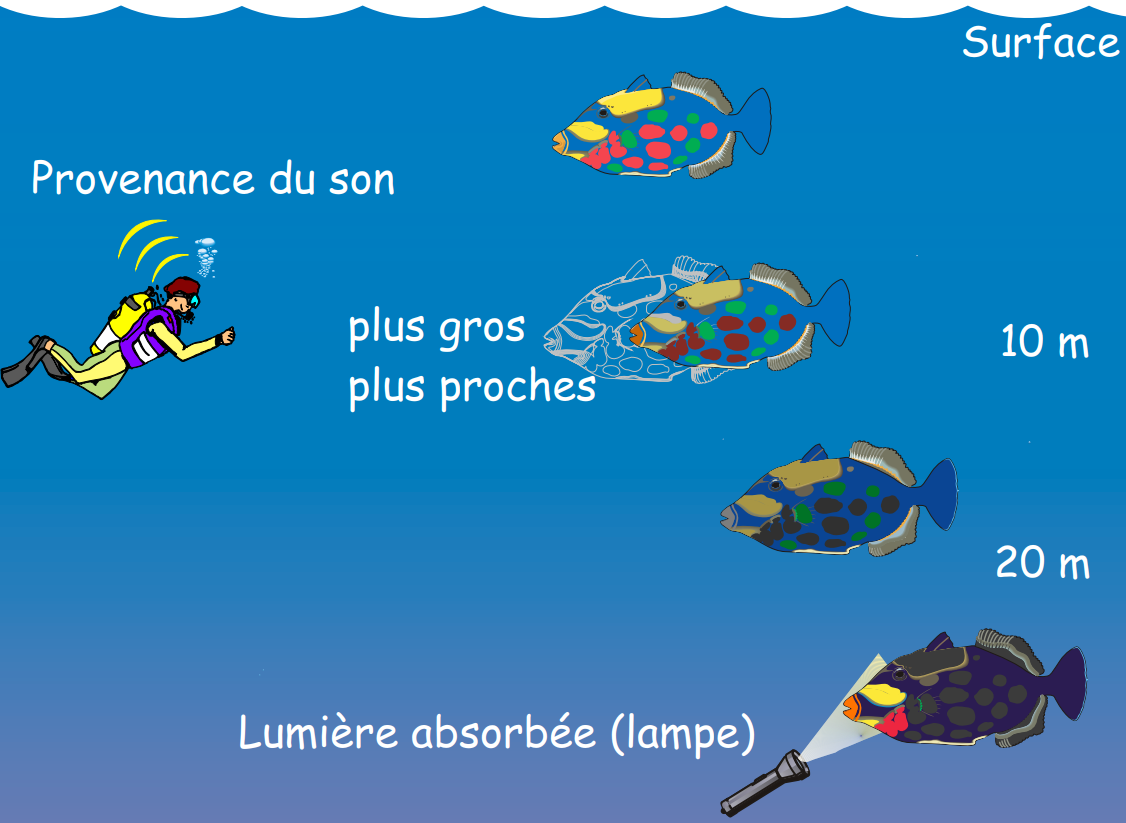
\includegraphics[width=\columnwidth,keepaspectratio]{images/sons-couleurs-dimensions}
  \end{columns}
\end{frame}
